% =====================================================================
%  English translation of
%    中: 基于生成式安全约束与闭环修正的扩散模型轨迹规划方法
%  Target layout: IEEE Robotics and Automation Letters (IEEEtran, journal)
%
%  Compile:  pdflatex main.tex   (no BibTeX: the source has no reference list)
% =====================================================================
\documentclass[journal]{IEEEtran}

\usepackage{amsmath}
\usepackage{amssymb}
\usepackage{amsfonts}
\usepackage{graphicx}
\usepackage{url}
\usepackage[hidelinks]{hyperref}
\usepackage{bm}

\graphicspath{{figures/}}

\newcommand{\R}{\mathbb{R}}
\newcommand{\ctrl}{H_{\mathrm{ctrl}}}
\newcommand{\ctrlf}{\widetilde{H}_{\mathrm{ctrl}}}
\newcommand{\hell}{H_{\mathrm{ell}}}
\newcommand{\Qraw}{\widehat{Q}_{0,\mathrm{raw}}^{(t)}}
\newcommand{\Qbdry}{\widehat{Q}_{0,\mathrm{bdry}}^{(t)}}
\newcommand{\Qalm}{Q_{0,\mathrm{ALM}}^{(t)}}
\newcommand{\abar}{\bar{\alpha}}

\begin{document}

\title{Diffusion-Based Trajectory Planning with Generative Safety
Constraints and Closed-Loop Correction}

\author{Author~Name,~\IEEEmembership{Member,~IEEE,}
        Author~Name,~\IEEEmembership{Member,~IEEE,}
        and~Author~Name,~\IEEEmembership{Senior~Member,~IEEE}%
\thanks{Manuscript received XXXX; revised XXXX.}}

\markboth{IEEE ROBOTICS AND AUTOMATION LETTERS. PREPRINT VERSION}%
{Author \MakeLowercase{\textit{et al.}}: Diffusion-Based Trajectory
Planning with Generative Safety Constraints and Closed-Loop Correction}

\maketitle

\begin{abstract}
Diffusion models offer a data-driven and multimodal way of generating
trajectories, yet the generation process itself cannot explicitly guarantee
trajectory safety. Existing safety-guided approaches focus mainly on guiding
and correcting a trajectory under a given constraint set, whereas work that
generates safety constraints from the environment structure and the planning
task, and then uses the resulting safety features to guide diffusion
denoising, remains limited. This paper proposes a diffusion-based trajectory
planning method with generative safety constraints and closed-loop
correction. Combining the environmental topology with local obstacle
information, the method generates a task-relevant convex safe corridor
through local ellipse prediction and convex region construction, and extracts
local safety features that guide diffusion denoising, while the convex safe
corridor supplies explicit safety constraints for trajectory correction.
During reverse diffusion, an augmented Lagrangian method corrects the
predicted control points, and the corrected result is used both for the
sampling state update and as historical feature feedback, forming a
closed-loop safety correction mechanism. Experiments on road scenes built in
CARLA show that, under identical test conditions, all compared methods
produce trajectory collisions to varying degrees, whereas the proposed method
exhibits no collision among any of the test trajectories, indicating superior
safety performance.
\end{abstract}

\begin{IEEEkeywords}
Diffusion-based trajectory planning, generative safety constraints, convex
safe corridor, closed-loop safety correction, augmented Lagrangian method.
\end{IEEEkeywords}

\section{Introduction}
\IEEEPARstart{B}{y} learning the probability distribution of trajectory data,
diffusion models provide a data-driven and multimodal means of trajectory
planning. They have already been applied to task-conditioned trajectory
generation and optimization: Diffuser generates goal-directed trajectories
under cost guidance, whereas MPD combines a learned trajectory prior with cost
gradients. Learning a trajectory distribution, however, does not by itself
ensure that the generated result satisfies the safety constraints of the
environment. In non-convex environments with complex obstacle layouts and
several feasible routes, a generated trajectory may depart from obstacle-free
space and thus incur a collision risk. Preserving the multimodal generative
capability of diffusion models while improving trajectory safety is therefore
a central problem for diffusion-based trajectory planning.

To improve safety, previous work has introduced explicit safety constraints
into the reverse diffusion process. SafeDiffuser, for instance, constrains
trajectory generation with control barrier functions (CBFs), and Projected
Diffusion Models correct infeasible predictions through projection-based
optimization. Such methods concentrate on how a given safety constraint is
used to guide or correct the generated trajectory; the constraint is usually a
predefined function or feasible set rather than one obtained by learning the
spatial structure of the environment. Moreover, the safety constraint acts on
the sampling process mainly through gradient guidance or optimization-based
correction, and the direct exploitation of local safety features inside the
denoising network has received comparatively little attention. How to generate
task-relevant safety constraints from the environmental topology and local
obstacle information, how to have the local safety features learned during
generation participate in diffusion denoising, and how to exploit the generated
constraints for continuous-trajectory correction are therefore the primary
questions addressed in this paper.

Beyond the generation and application of safety constraints, the way
historical correction information is exploited across the multi-step reverse
diffusion process also warrants attention. Existing constraint-guided and
optimization-based methods can correct the current predicted trajectory and
influence subsequent generation through the sampling state update, but the
earlier correction is not necessarily supplied to the denoising network as an
explicit condition. Subsequent predictions may therefore repeat similar
constraint violations and require the safety correction to be executed again.
How to incorporate historical safety corrections into the conditioning
representation of the denoising network, so that they affect not only the
sampling state update but also subsequent trajectory prediction, is the second
question addressed here.

To address these questions, this paper proposes TrajSafe-Diffuser, a
diffusion-based trajectory planning method with generative safety constraints
and closed-loop correction. For the construction of generative safety
constraints, feasible routes are selected from the free space of the
environment according to the planning task, local ellipse parameters are
predicted along the selected route, and a task-relevant convex safe corridor is
obtained by convex region construction. Unlike approaches that merely use a
given constraint to guide or correct a trajectory, local safety features are
learned together with the safety constraints and serve as conditioning
information for the denoising network, while the generated convex safe corridor
establishes explicit safety constraints, so that environment- and task-related
safety information acts separately on trajectory prediction and on constraint
correction.

For closed-loop safety correction, the generated convex safe corridor
constrains the trajectory predicted by reverse diffusion, and an augmented
Lagrangian method corrects the predicted control points. Rather than using the
corrected result only for the sampling state update, a historical safety
feedback mechanism is designed that injects the corrected control points and
their change into the subsequent denoising network in a gated manner, so that
the denoising prediction can exploit earlier safety corrections and a closed
loop is formed between trajectory generation and safety correction.

The main contributions of this paper are as follows.
\begin{enumerate}
\item \emph{A diffusion-based trajectory planning framework with generative
safety constraints and closed-loop correction.} Aiming at safe trajectory
generation in complex non-convex environments, it combines task-relevant safety
constraint generation with diffusion-based trajectory planning, yielding a
framework that integrates safety-conditioned guidance, explicit constrained
optimization and historical feedback.

\item \emph{A generative safety constraint construction method for complex
non-convex environments.} Candidate routes are matched against the
environmental topology and the planning task; local ellipse parameter
prediction together with convex region construction produces a task-relevant
convex safe corridor, and local safety features are learned simultaneously, so
that the generated safety information can be used separately for diffusion
denoising guidance and for continuous-trajectory constraint correction.

\item \emph{A closed-loop safety correction mechanism based on constrained
optimization and historical feedback.} The augmented Lagrangian method corrects
the predicted control points during reverse diffusion and the result updates
the subsequent sampling state, while a gating mechanism injects the historical
correction into the denoising network so that earlier safety corrections
participate in later trajectory prediction.
\end{enumerate}

\section{Problem Definition}

Consider trajectory planning in a two-dimensional static environment. Given an
occupancy grid map $O\in\{0,1\}^{H\times W}$, a start $\bm S\in\R^2$ and a
goal $\bm G\in\R^2$, the objective is to generate a continuous trajectory that
connects the start and the goal while satisfying the obstacle-avoidance
requirement of the environment.

The trajectory is represented by a clamped cubic B-spline defined by
$C=48$ control points. Denoting the control point set by
$Q=[q_0,\ldots,q_{C-1}]\in\R^{C\times2}$, the continuous trajectory is
\begin{equation}
\tau_Q(u)=\sum_{j=0}^{C-1}B_{j,3}(u)\,q_j,\qquad u\in[0,1],
\end{equation}
where $B_{j,3}$ is the cubic B-spline basis function and $u$ the curve
parameter. Owing to the endpoint interpolation property of clamped B-splines,
$q_0=\bm S$ and $q_{C-1}=\bm G$ are fixed and diffusion sampling is performed
only on the interior control points.

Let $\mathcal F(O)$ denote the obstacle-free space of the map. The trajectory
is then required to satisfy
\begin{equation}
q_0=\bm S,\quad q_{C-1}=\bm G,\quad
\tau_Q(u)\in\mathcal F(O),\quad \forall u\in[0,1].
\end{equation}
A conditional diffusion model is used to learn the control point distribution
$p_\theta(Q\mid O,\bm S,\bm G)$ and thereby generate different candidate
trajectories. Since probabilistic modeling cannot directly guarantee the
continuous obstacle-avoidance condition above, this paper further studies how
to generate safety constraints from the environment structure and the planning
task, and how to improve the safety feasibility of the generated trajectory
through constraint correction and historical feedback during reverse diffusion.

\section{Method}

The overall structure of TrajSafe-Diffuser is shown in Fig.~\ref{fig:framework}.
It comprises three modules: feature encoding and fusion, generative safety
constraint construction, and trajectory denoising with closed-loop correction.
The model first encodes the environment, the current noisy control points and
the historical feedback into conditioning features used for route matching and
trajectory prediction. Candidate route matching, local ellipse prediction and
convex region construction then generate the safety constraints, and local
safety features are extracted to guide denoising. Finally, the
reverse-diffusion prediction, after explicit constraint correction, takes part
in subsequent generation through the sampling state update and the historical
feedback.

\begin{figure*}[!t]
\centering
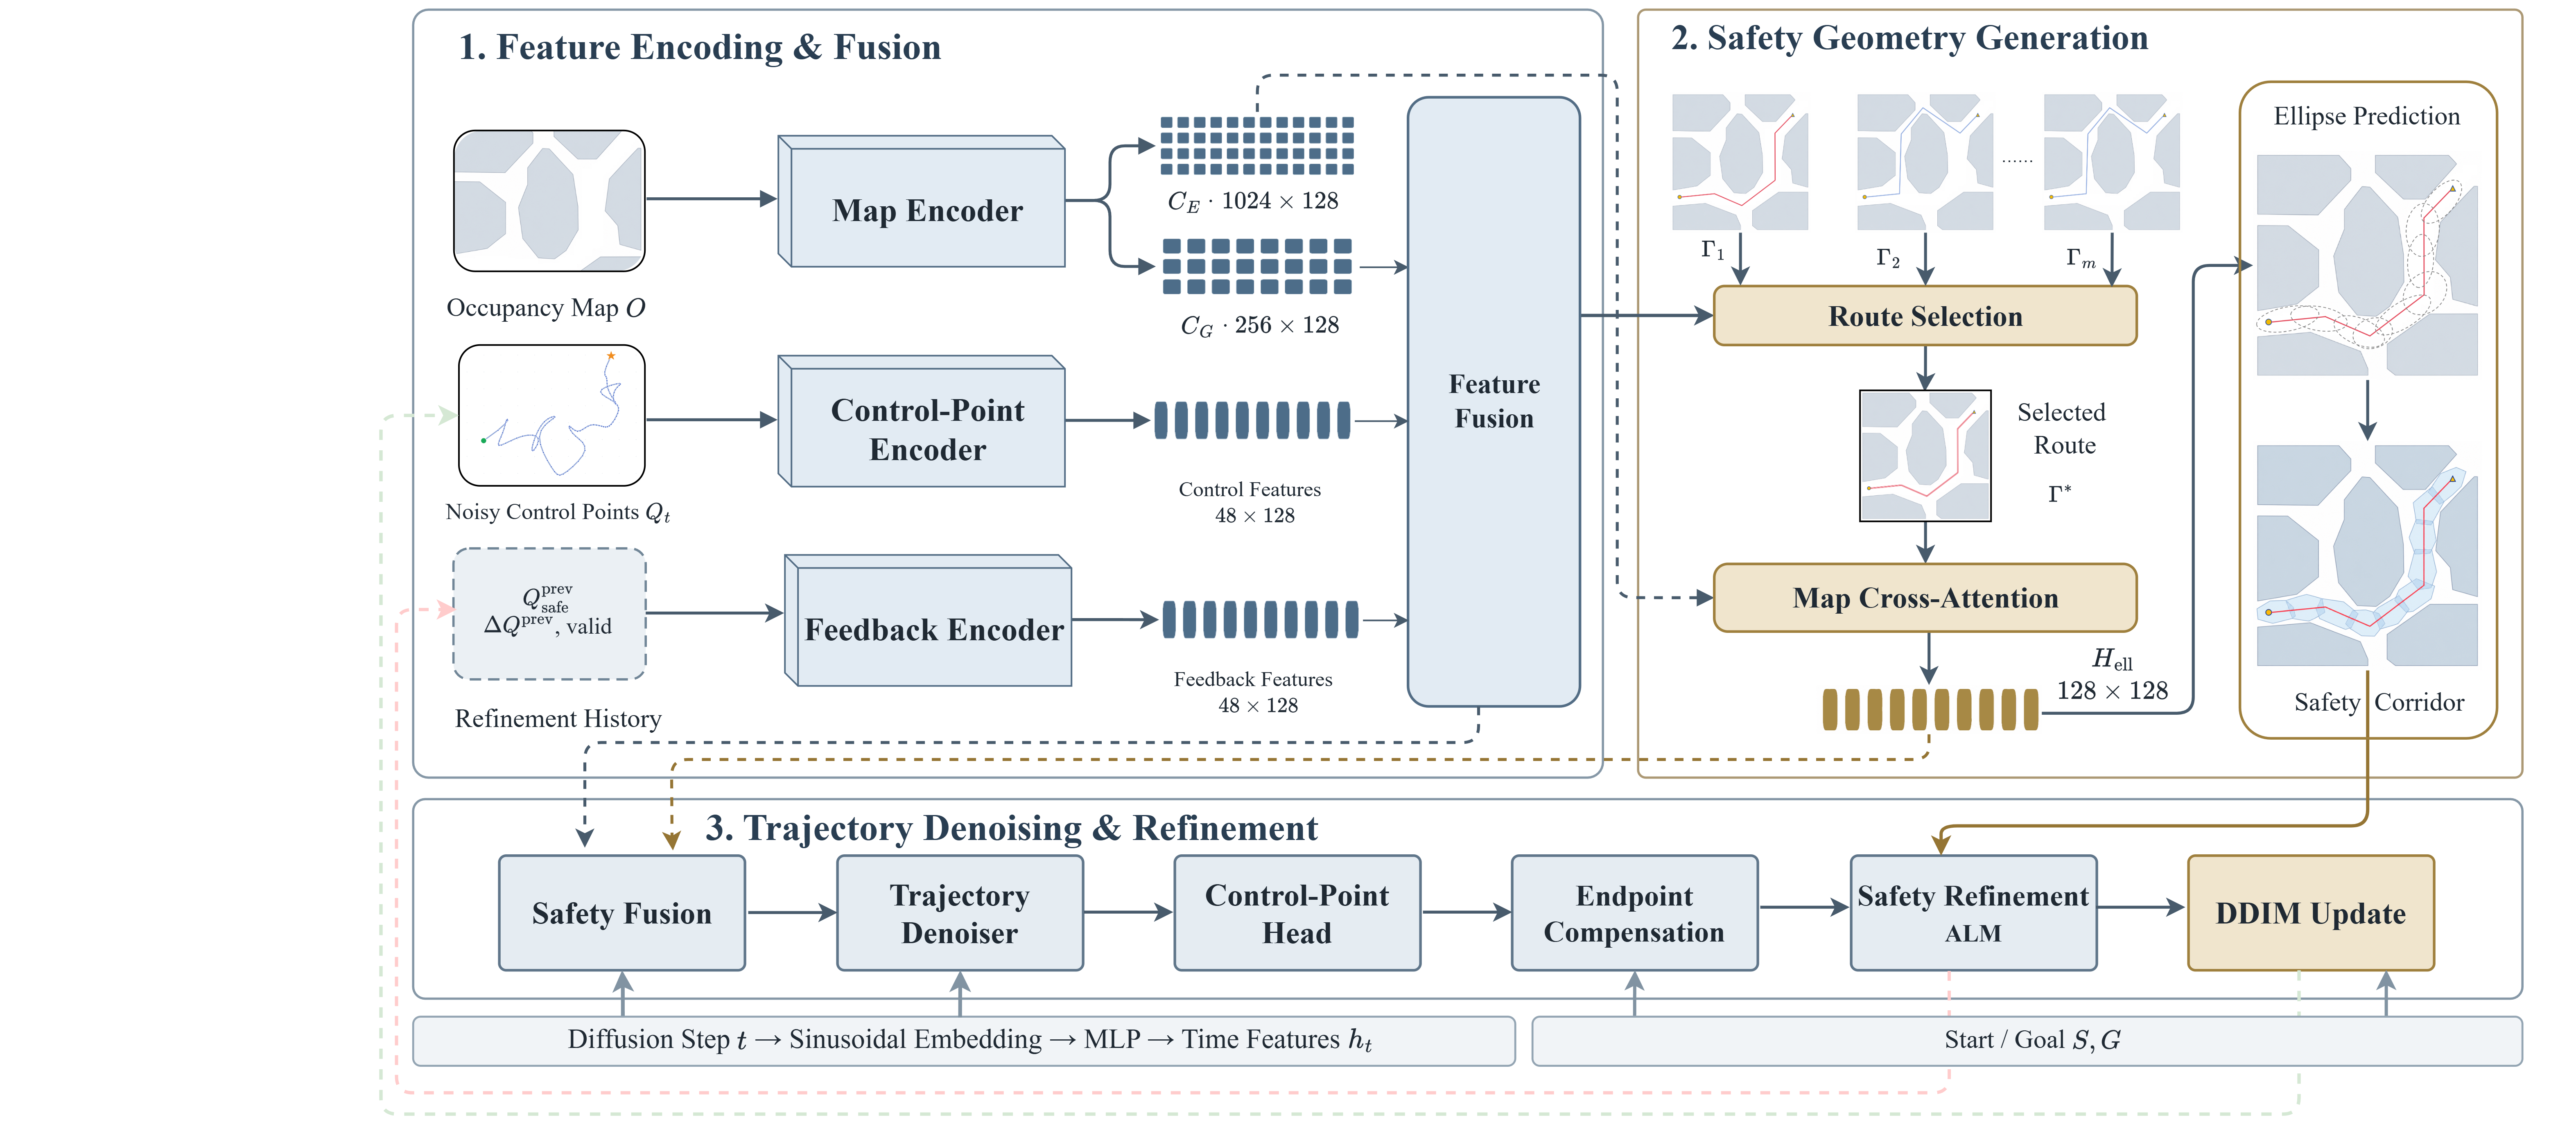
\includegraphics[width=0.85\textwidth]{fig1_framework.png}
\caption{Overall framework of TrajSafe-Diffuser.}
\label{fig:framework}
\end{figure*}

Diffusion acts only on the interior control points. During training, Gaussian
noise is added to the reference interior control points according to the
cumulative signal coefficient $\abar_t$; during inference, sampling starts from
Gaussian noise and clean control points are predicted through multi-step
reverse diffusion, with the first and last control points held fixed
throughout.

\subsection{Feature Encoding and Fusion}

The feature encoding module converts the occupancy map, the noisy control
points and the diffusion time step into a unified feature representation, and
fuses historical safety correction information through a gating mechanism,
providing conditioning inputs for the subsequent safety constraint generation
and trajectory denoising.

\subsubsection{Map and Control Point Feature Encoding}

A multi-scale convolutional encoder--decoder network is used to extract map
features. The encoder obtains global map features through successive
downsampling, and the decoder upsamples and fuses intermediate features to
produce map features that retain local spatial information. After channel
mapping and spatial positional encoding, the two branches yield a global map
feature $C_G\in\R^{256\times128}$ and a local map feature
$C_E\in\R^{1024\times128}$, corresponding to spatial resolutions of
$16\times16$ and $32\times32$. $C_G$ is used for control point feature
encoding and conditional denoising, whereas $C_E$ is used for local safety
feature extraction.

For the current noisy control points $Q_t$, the coordinates are first
positionally encoded and mapped by an MLP, and a control point index encoding
is then added, giving the initial control features
\begin{equation}
X_j^{(0)}
=\operatorname{MLP}_{T}\!\left(\Phi_{xy}(q_{t,j})\right)
+\operatorname{PE}_{1D}(j).
\end{equation}
Eight conditional attention blocks are then applied to extract the relations
among control points and the environment information. Each block consists of
control point self-attention, global-map cross-attention and a feed-forward
network, and the diffusion time condition is introduced through adaptive layer
normalization. Four attention heads and 128-dimensional features are used,
yielding
\begin{equation}
\ctrl\in\R^{48\times128}.
\end{equation}

\subsubsection{Historical Safety Feedback Fusion}

To let the denoising network exploit earlier safety corrections, the most
recent corrected control points that passed the acceptance check,
$Q_{\mathrm{hist}}$, the corresponding correction $\Delta Q_{\mathrm{hist}}$
and a feedback validity flag $v\in\{0,1\}$ are taken as historical feedback
inputs. The resulting five-dimensional feedback vector of each control point is
encoded by an MLP into
$H_{\mathrm{fb}}\in\R^{48\times128}$.

Since different control points and feature channels depend on the historical
correction to different degrees, a channel-wise gating mechanism is used for
fusion:
\begin{equation}
\begin{aligned}
g&=\sigma\!\left(W_g[\ctrl;H_{\mathrm{fb}}]+b_g\right),\\
\ctrlf&=\ctrl+v\,g\odot H_{\mathrm{fb}},
\end{aligned}
\end{equation}
where $[\cdot;\cdot]$ denotes feature concatenation, $\sigma$ the sigmoid
function and $\odot$ the element-wise product, with
$g\in\R^{48\times128}$. When no valid historical feedback exists, $v=0$ and
the control features are unaffected by the feedback branch; otherwise the
historical correction is fused adaptively according to the gating weights.

The fused control features $\ctrlf$ are used both for the subsequent candidate
route matching and for conditional denoising, so that the historical safety
correction contributes to the feature computation of both stages.

\subsection{Generative Safety Constraint Construction}

Based on the environmental topology and the local obstacle information, the
generative safety constraint module learns task-relevant safety features and
builds the convex safe corridor used for trajectory correction. It consists of
two main stages: candidate route matching, and local ellipse prediction with
convex region construction.

\subsubsection{Candidate Route Matching and Selection}

At most $M$ candidate routes $\{\Gamma_m\}_{m=1}^{M}$ are first extracted from
the free space of the environment and, after equal-arclength resampling and
feature encoding, represented as $H_{S,m}\in\R^{128\times128}$.

With the fused control features $\ctrlf$ as queries and the candidate route
features as keys and values, time-conditioned cross-attention computes the
matching features between the control points and each candidate route. Average
pooling over the control point dimension followed by a scoring network and a
masked softmax then gives the route selection probabilities $\pi_m$.

The highest-scoring candidate is selected first; if the corresponding safe
corridor cannot be constructed, the remaining valid candidates are tried in
turn. Once a safe corridor has been built, the selected route $\Gamma^*$ and
its features are frozen, so that the route and the safety constraint stay
consistent in the later sampling steps.

\subsubsection{Local Safety Feature Extraction and Convex Safe Corridor Construction}

Along the selected route $\Gamma^*$, $N_q=128$ fixed centers $c_i$ are sampled
at equal arc length. Using the route features as queries, the corresponding
obstacle information is extracted from the local map features $C_E$. To
strengthen the network's attention to the spatial structure near the safety
centers, a distance bias is added to the cross-attention scores:
\begin{equation}
\mathcal B_{ij}^{\mathrm{geo}}
=\operatorname{clip}\!\left(
-\frac{\abar_t\,\lVert c_i-z_j\rVert_2^2}
{2\sigma_{\mathrm{geo}}^2},
-b_{\mathrm{clip}},0\right),
\end{equation}
where $z_j$ is the spatial position corresponding to map feature $j$, and
$\sigma_{\mathrm{geo}}$ and $b_{\mathrm{clip}}$ control the distance decay
scale and the clipping range, respectively.

The distance-biased cross-attention yields the local safety features
$\hell\in\R^{128\times128}$, from which an ellipse prediction head outputs the
local ellipse parameters
\begin{equation}
e_i=(\log a_i,\ \log b_i,\ \cos 2\theta_i,\ \sin 2\theta_i).
\end{equation}
The ellipse center is determined by the selected route, and the network predicts
only its scale and orientation. The predicted ellipse provides a geometric
prior of the local space but does not by itself guarantee obstacle-free space.

Using the predicted ellipse as geometric prior, a deterministic convex region
construction is then carried out according to the obstacle grid, the map
boundary and a safety margin, giving the local obstacle-free convex region
\begin{equation}
\mathcal R_i=\{x\in\R^2\mid A_ix\leq b_i\}.
\end{equation}
Obstacle intersection checks, overlap checks between adjacent regions and, where
necessary, region bridging produce the convex safe corridor $\mathcal C$
arranged along the selected route.

The generative safety constraint module thus yields two interrelated
representations: \emph{the local safety features $\hell$ guide diffusion
denoising, while the convex safe corridor $\mathcal C$ provides explicit safety
constraints for the continuous trajectory.}

\begin{figure*}[!t]
\centering
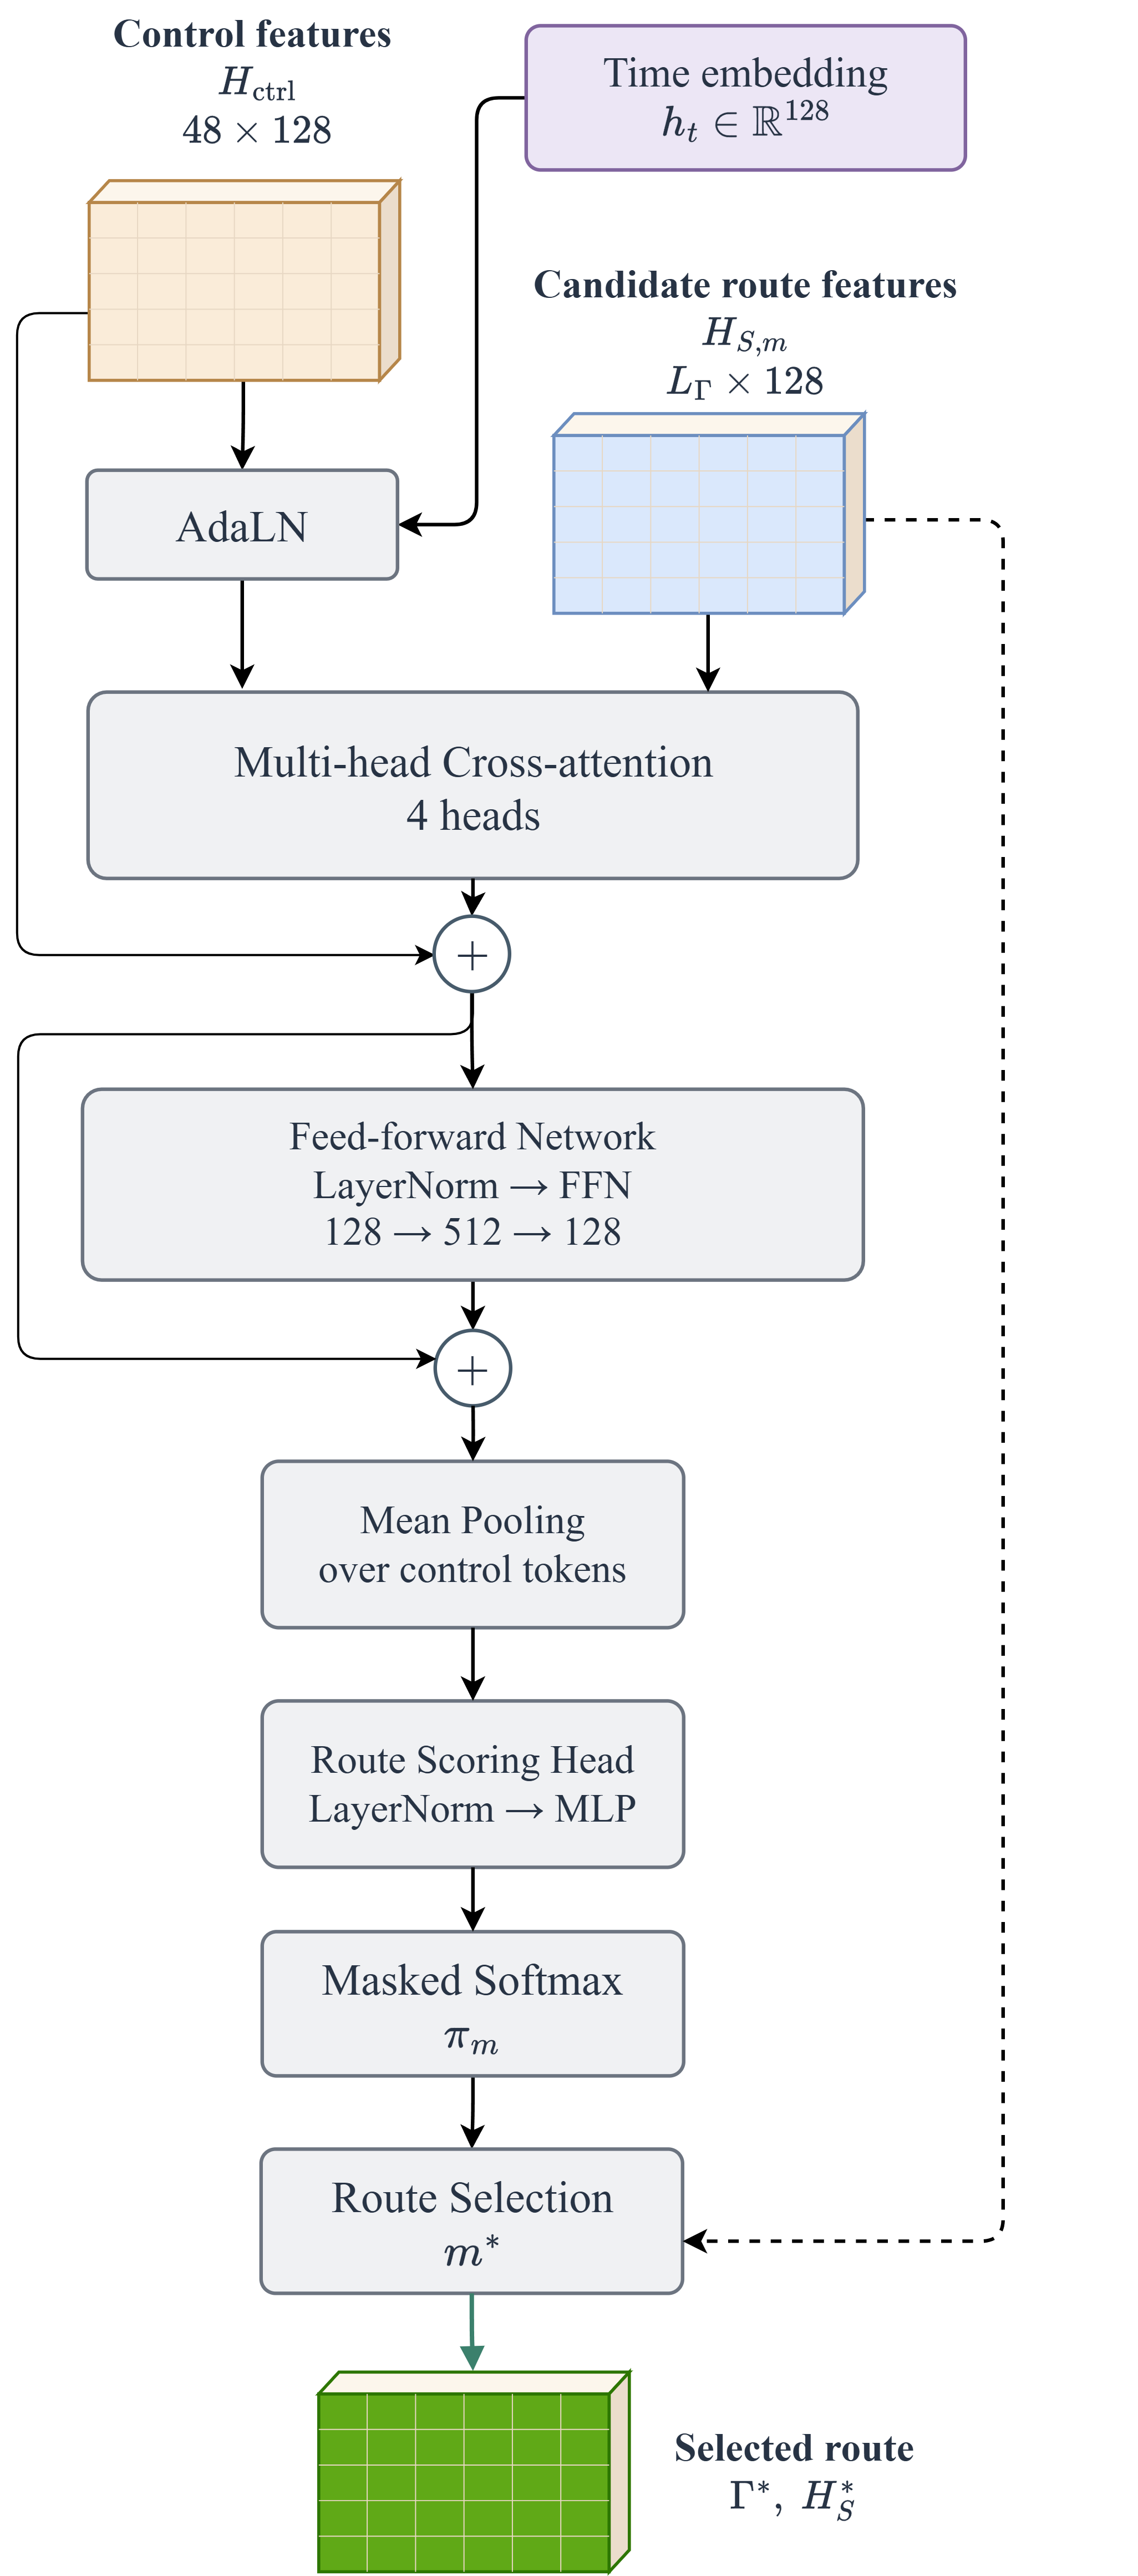
\includegraphics[width=0.34\textwidth]{fig2a_safety_generation_route.png}\\[3pt]
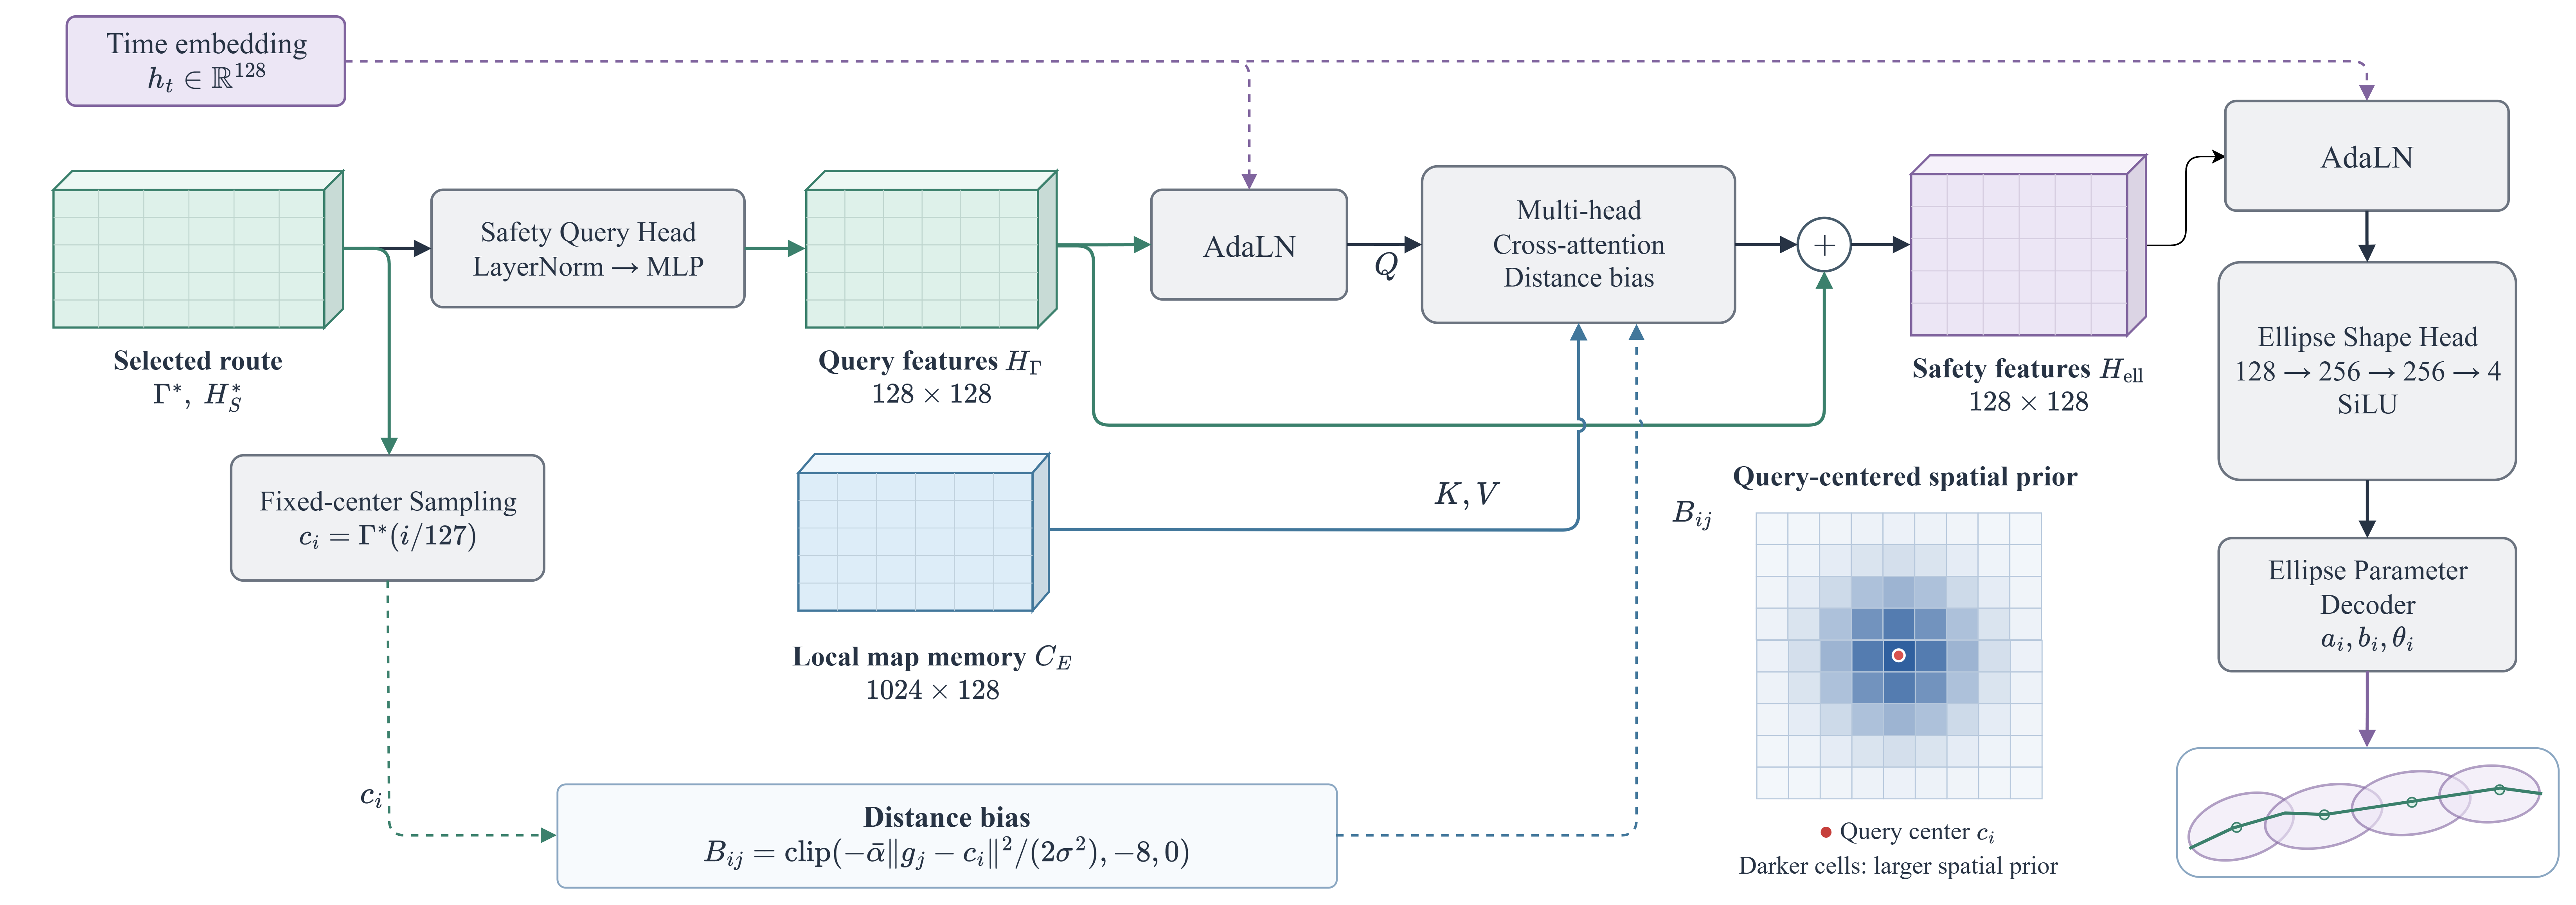
\includegraphics[width=0.85\textwidth]{fig2b_safety_generation_geometry.png}
\caption{Generative safety constraint construction. (a) Candidate route
matching and selection. (b) Local safety feature extraction, ellipse
prediction and convex region construction.}
\label{fig:safety}
\end{figure*}

\subsection{Trajectory Denoising and Closed-Loop Safety Correction}

Building on the generative safety constraints, the local safety features are
introduced into the diffusion denoising network so as to produce a trajectory
prediction consistent with the selected route. The generated convex safe
corridor then constrains the continuous trajectory, and the corrected result is
fed back into the subsequent reverse diffusion process.

\subsubsection{Safety-Conditioned Denoising and Endpoint Compensation}

With the fused control features $\ctrlf$ obtained in Section~III-A as queries,
multi-head cross-attention extracts the information relevant to each control
point from the local safety features $\hell$. Residual fusion followed by an
MLP mapping gives the safety-conditioned control features
$F\in\R^{48\times128}$. $F$ is then fed to three conditional denoising blocks
that predict the clean control points $\Qraw$, conditioned on the global map
features $C_G$ and the diffusion time step $t$. Each block contains control
point self-attention, map cross-attention and a feed-forward network, and the
time condition is introduced through adaptive layer normalization.

To satisfy the fixed start and goal, the prediction errors of the first and
last control points are compensated to the neighbouring control points with
preset weights, after which the two endpoints are set to $\bm S$ and $\bm G$,
giving the endpoint-compensated control points $\Qbdry$. This satisfies the
endpoint constraints while reducing the local change of trajectory shape caused
by replacing the endpoints directly.

\subsubsection{Continuous-Trajectory Safety Constraint and ALM Correction}

The convex safe corridor consists of several local convex regions arranged
along the selected route, whereas the diffusion model outputs one entire
B-spline curve defined by $C=48$ control points. Although a cubic B-spline has
the local convex-hull property, building the safety constraint directly on the
original control points would generally require the four control points
affecting a given curve segment to be confined to the same convex region
simultaneously. Because the local convex regions are densely distributed along
the route, their coverage need not match the convex hull of the original
control points, and such a constraint easily becomes overly conservative. To
make the safety constraint correspond to a shorter continuous curve segment,
the B-spline is first refined parametrically, and each subsegment is then
converted exactly into a cubic B\'ezier curve.

Specifically, let the convex safe corridor contain $N$ convex regions ordered
by route progress, and let $s_i\in[0,1]$ be the normalized progress along the
selected route of the reference position associated with region $i$.
Responsibility intervals are delimited by the progress midpoints of adjacent
regions:
\begin{equation}
m_i=\frac{s_i+s_{i+1}}{2},\ \ i=1,\ldots,N-1,
\qquad m_0=0,\quad m_N=1.
\end{equation}
Region $i$ therefore corresponds to the curve-parameter interval
$[m_{i-1},m_i]$. This establishes a preset correspondence between route
progress and curve parameter; the curve is not required to already lie inside
the region before correction. Since a cubic B-spline is a single cubic
polynomial only between adjacent knots, an interval crossing a knot cannot be
represented exactly by one set of cubic B\'ezier control points. The interval
boundaries are therefore merged with the B-spline knots, sorted and
de-duplicated, yielding $K$ final subsegments. Each subsegment corresponds to
one convex region and does not cross a B-spline knot, and can hence be
converted exactly into a cubic B\'ezier curve.

Let the parameter interval of subsegment $k$ be $[u_{k-1},u_k]$, of length
$h_k=u_k-u_{k-1}$, and let $Q\in\R^{C\times2}$ be the control point matrix of
the original B-spline. The four B\'ezier control points of the subsegment
satisfy
\begin{equation}
\bm\beta_k=E_kQ,
\end{equation}
where $\bm\beta_k\in\R^{4\times2}$ and $E_k\in\R^{4\times C}$. Denoting by
$\mathbf n(u)\in\R^{1\times C}$ the row vector of B-spline basis functions and
by $\mathbf n'(u)$ its derivative, the conversion matrix is determined by the
position and the first derivative at both ends of the subsegment:
\begin{equation}
E_k=
\begin{bmatrix}
\mathbf n(u_{k-1})\\[2pt]
\mathbf n(u_{k-1})+\dfrac{h_k}{3}\mathbf n'(u_{k-1})\\[4pt]
\mathbf n(u_k)-\dfrac{h_k}{3}\mathbf n'(u_k)\\[4pt]
\mathbf n(u_k)
\end{bmatrix}.
\end{equation}
At a B-spline knot the one-sided derivative corresponding to the interior of the
subsegment is used. This conversion does not alter the shape of the original
curve, and the B\'ezier control points are determined linearly by $Q$, so no
additional optimization variable is introduced.

Owing to the convex-hull property of B\'ezier curves, if the four B\'ezier
control points of a subsegment all lie inside their corresponding convex safe
region, the whole continuous curve segment lies inside that region. Writing the
convex region of subsegment $k$ as
\begin{equation}
\mathcal R_k=\{x\in\R^2\mid A_kx\leq b_k\},
\end{equation}
the safety constraint becomes
\begin{equation}
A_k\bm\beta_{k,j}\leq b_k,\qquad j=1,2,3,4,
\end{equation}
where $\bm\beta_{k,j}\in\R^2$ is the $j$-th B\'ezier control point of segment
$k$. Substituting $\bm\beta_k=E_kQ$ gives linear inequalities in the original
B-spline control points $Q$. Collecting the constraints of all subsegments as
$g(Q)\leq0$ and noting that every convex region has already passed the obstacle
separation and validity checks, satisfying these constraints keeps the whole
continuous trajectory inside its assigned safety region, rather than merely
ensuring that a finite set of sample points is collision-free. It should be
emphasized that this is a sufficient condition for continuous safety; the
assignment of parameter intervals to convex regions does not by itself
guarantee that the optimization problem is feasible.

As shown in Fig.~\ref{fig:alm}, the augmented Lagrangian method (ALM) is used to
adjust the original B-spline control points, satisfying the continuous safety
constraint while preserving the shape of the predicted trajectory as far as
possible. Taking the endpoint-compensated result
$Q^{\mathrm{ref}}=\Qbdry$ as reference and defining
$\Delta Q=Q-Q^{\mathrm{ref}}$, the optimization problem is
\begin{equation}
\begin{aligned}
\min_{Q}\quad
&\frac{\lambda_p}{2}\lVert\mathbf B\Delta Q\rVert_F^2
+\frac{\lambda_s}{2}\lVert D_2\mathbf B\Delta Q\rVert_F^2\\
\mathrm{s.t.}\quad
&g(Q)\leq0,\\
&q_0=\bm S,\qquad q_{C-1}=\bm G,
\end{aligned}
\end{equation}
where $\mathbf B$ is the B-spline sampling basis matrix, $D_2$ the
second-difference matrix, and $\lambda_p$ and $\lambda_s$ weighting
coefficients. The first term limits the positional offset introduced by the
correction and the second suppresses local fluctuation of the correction along
the trajectory. Holding the endpoints fixed, the ALM iteratively updates the
interior control points and the constraint multipliers to obtain $\Qalm$. The
maximum safety constraint violation is then computed in order to judge whether
the correction is valid; if the constraint tolerance is not met, the result is
not accepted as new valid historical feedback.

\begin{figure*}[!t]
\centering
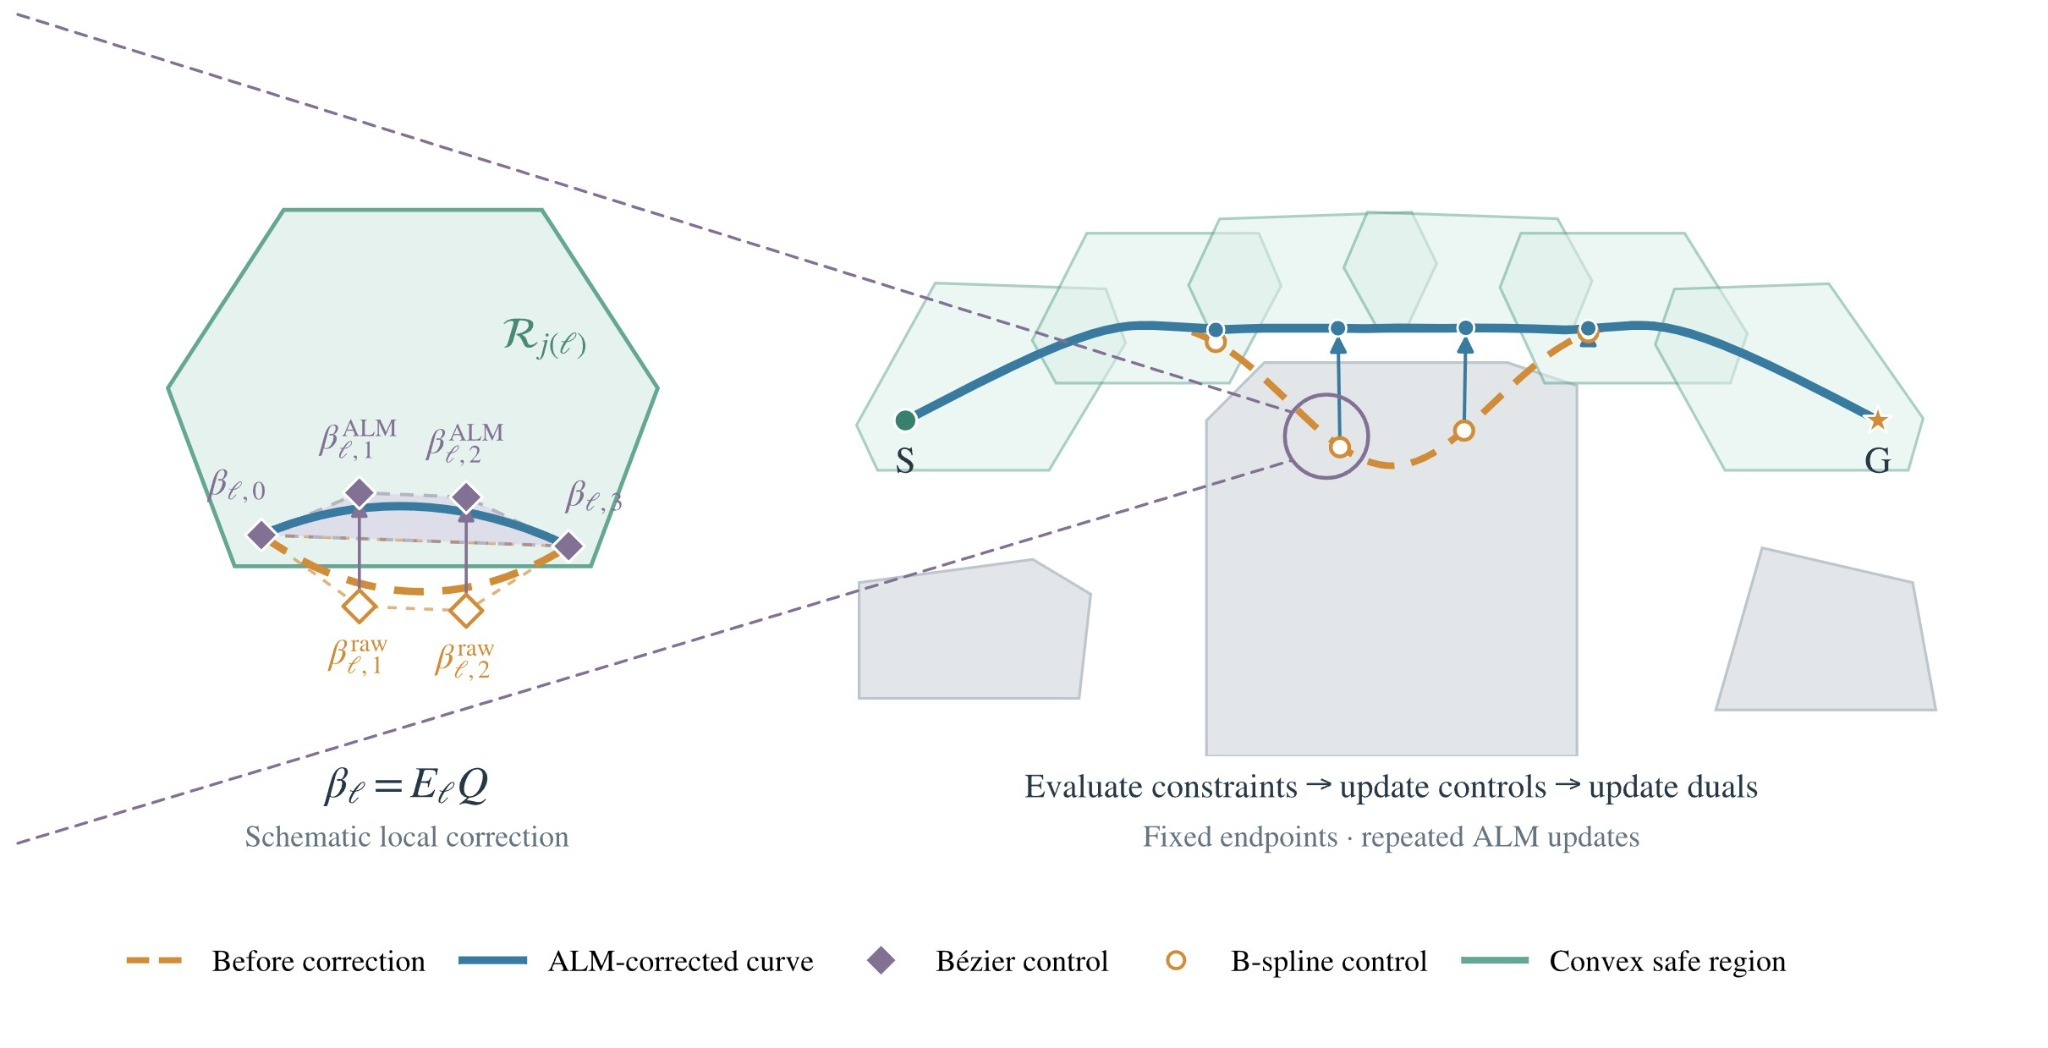
\includegraphics[width=0.68\textwidth]{fig3_alm.jpg}
\caption{Continuous-trajectory safety constraint and ALM correction. Left:
constraint relation between the B\'ezier control points of a curve subsegment
and the corresponding convex region. Right: change of the trajectory under
fixed start and goal before and after ALM correction.}
\label{fig:alm}
\end{figure*}

\subsubsection{Reverse-Diffusion State Update and Historical Feedback}

The safety correction result enters the subsequent reverse diffusion through
two paths: the sampling state update and the historical feature feedback.
First, the corrected control points $\Qalm$ are taken as the clean control
point estimate at the current step, the noise is recomputed, and a
deterministic DDIM update is performed:
\begin{equation}
\begin{aligned}
\widehat{\epsilon}_t
&=\frac{Q_t-\sqrt{\abar_t}\,\Qalm}{\sqrt{1-\abar_t}},\\
Q_s&=\sqrt{\abar_s}\,\Qalm+\sqrt{1-\abar_s}\,\widehat{\epsilon}_t,
\qquad 0\leq s<t,
\end{aligned}
\end{equation}
where $\abar_t$ and $\abar_s$ are the cumulative signal coefficients of the
corresponding time steps. The state update acts only on the interior control
points, the first and last control points remain fixed, and the final
reverse-diffusion step directly adopts the corrected clean control point
prediction.

Second, for corrections that pass the constraint check, the corrected control
points and their change with respect to the endpoint-compensated prediction are
stored:
\begin{equation}
\begin{aligned}
Q_{\mathrm{hist}}&=\Qalm,\\
\Delta Q_{\mathrm{hist}}&=\Qalm-\Qbdry.
\end{aligned}
\end{equation}
If the correction fails the check, the existing valid historical feedback is
not overwritten. At the next reverse-diffusion step, the cached control points
and correction are fed again into the gated fusion module of
Section~III-A, so that the network can exploit the previous round of safety
correction in subsequent prediction. The DDIM update therefore changes the
subsequent sampling state directly, while the historical feedback makes the
safety correction participate in subsequent denoising; together they close the
loop between trajectory prediction and constraint correction.

\subsection{Training Strategy and Loss Function}

To enable the denoising network to learn to exploit the historical correction
information, a two-forward training strategy with shared parameters is adopted.

First, a diffusion time step $t$ is sampled at random, noise is added to the
reference control points to obtain $Q_t$, and the first network forward pass is
carried out without historical feedback. The offline convex safe corridor
associated with the reference route is then used for ALM correction, and the
historical control points, the correction and the validity flag are constructed
from the constraint-residual check. When the prediction already satisfies the
constraints the correction is set to zero; when the correction fails the
acceptance check the feedback flag is set invalid. One DDIM update is performed
with the correction, giving the noisy control points at the next time step.

The second forward pass receives the updated control points and the constructed
historical feedback, and uses the same network parameters as the first pass.
The ALM solve, the residual check, the feedback construction and the DDIM
update all stop gradient propagation, so that gradients from the second
prediction do not back-propagate to the first prediction through these steps.
During training, part of the historical feedback is masked at random in order
to accommodate the absence of valid feedback early in inference.

The training loss consists of three parts: trajectory prediction, safety
constraint generation and safety constraint satisfaction.

The trajectory prediction losses comprise the control point reconstruction loss
$\mathcal L_{\mathrm{ctrl}}$, the endpoint-neighbourhood loss
$\mathcal L_{\mathrm{boundary}}$ and the control point smoothness loss
$\mathcal L_{\mathrm{smooth}}$, which constrain the trajectory prediction error
and the local shape change.

The safety constraint generation losses comprise the route classification loss
$\mathcal L_{\mathrm{topo}}$, the ellipse shape loss
$\mathcal L_{\mathrm{shape}}$, the region overlap loss
$\mathcal L_{\mathrm{IoU}}$ and the ellipse safety loss
$\mathcal L_{\mathrm{safe}}$, supervising candidate route selection, ellipse
parameter prediction, region coverage and the degree of obstacle intrusion,
respectively.

The safety constraint satisfaction losses comprise the corridor loss
$\mathcal L_{\mathrm{alm}}$ and the continuous safety loss
$\mathcal L_{\mathrm{fb,safe}}$. The former is computed from the corridor
violation of sample points on the first predicted trajectory; the latter
measures, for the second prediction, the continuous-curve constraint violation
through the B\'ezier control point inequalities. A curve smoothness loss
$\mathcal L_{\mathrm{curve}}$ is additionally applied to the decoded trajectory
of the second prediction. These losses are combined with preset weights to form
the complete training objective.

\end{document}
